%%%%%%%%%%%%%%%%%%%%%%%%%%%%%%%%%%%%% 
%% LE2I beamer template
%% Guillaume Lemaitre, October 2014
%%%%%%%%%%%%%%%%%%%%%%%%%%%%%%%%%%%%% 

\documentclass{beamer}

\usepackage[utf8]{inputenc}
\usepackage[T1]{fontenc} 
\usetheme{le2i} 

%% The amssymb package provides various useful mathematical symbols
\usepackage{amssymb}
%% The amsthm package provides extended theorem environments
\usepackage{amsthm}

%% amsmath for math environment
\usepackage{amsmath}

\DeclareMathOperator*{\argmin}{arg\,min}
\DeclareMathOperator*{\argmax}{arg\,max}
\DeclareMathOperator*{\sign}{sign}

%% figure package
\usepackage{epsf,graphicx}
\usepackage{epstopdf}
\usepackage{subfigure}
\usepackage{transparent}

%% In order to draw some graphs
\usepackage{tikz,xifthen}
\usepackage{tikz-qtree}
\usepackage{adjustbox}
\usetikzlibrary{decorations.pathmorphing}
\usetikzlibrary{fit}
\usetikzlibrary{backgrounds}
\usetikzlibrary{shapes,arrows,shadows}
\usetikzlibrary{calc,decorations.pathreplacing,decorations.markings,positioning}
\usetikzlibrary{snakes,decorations.text,shapes,patterns}
% \usepackage{scalefnt,lmodern,booktabs}

%% Package for cross and tick symbols
\usepackage{pifont}
\newcommand{\tick}{\color{green!60!black!80}\ding{51}}
\newcommand{\cross}{\color{red!60!black!80}\ding{55}}

\title{Demosaicing}
\author{Guillaume Lemaitre}
%\date{Define the event \\ day\textsuperscript{th} Month Year}

\institute{Universit\'e de Bourgogne} 

%% Uncomment if you want to avoid thousand of bullet inside the menu
% \usepackage{etoolbox}
% \makeatletter
% \patchcmd{\slideentry}{\advance\beamer@xpos by1\relax}{}{}{}
% \def\beamer@subsectionentry#1#2#3#4#5{\advance\beamer@xpos by1\relax}%
% \makeatother

\begin{document}

% Show the title page
\begin{frame}
  \titlepage
\end{frame}

% Show the table of contents
\begin{frame}
  \tableofcontents[sectionstyle=show,subsectionstyle=show,subsubsectionstyle=hide]
\end{frame}

%---------------
\section{Color imaging}
\begin{frame}
\frametitle{Tri-CCD}
\begin{center}
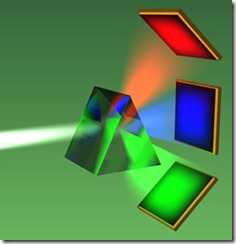
\includegraphics[scale= 0.8]{images/L7_triCCD.jpg}
\end{center}
\footnotesize{
\begin{itemize}
\item {\color{blue}
Good spatial resolution
\item Good color separation}
\item {\color{red}Expensive
\item Problem of channel alignment}

\end{itemize}
}
\end{frame}
%---------------
\begin{frame}
\frametitle{Tri-CCD}
\begin{center}
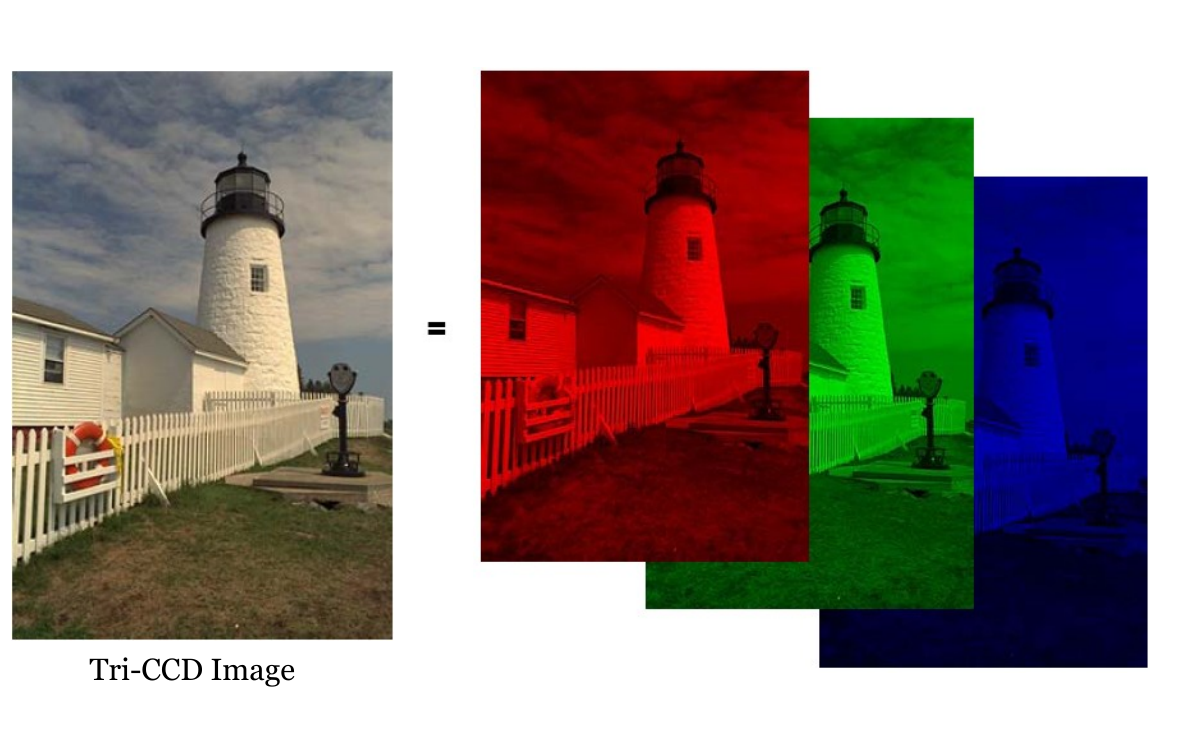
\includegraphics[scale=0.35]{images/L7_ex_triCCD.png}
\end{center}
\end{frame}
%---------------
\begin{frame}
\frametitle{Mono CCD: CFA}
\begin{center}
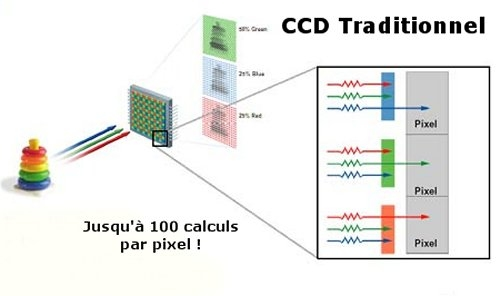
\includegraphics[scale= 0.45]{images/L7_monoCCD.jpg}\\
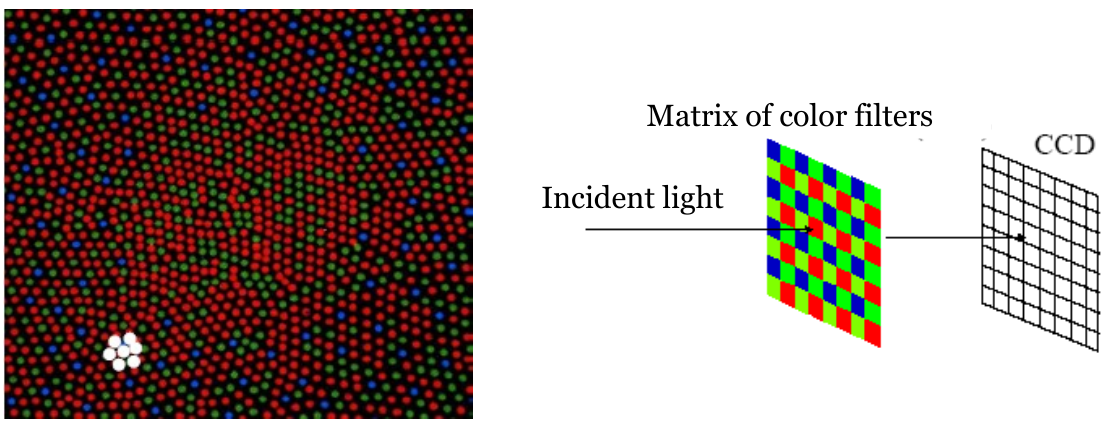
\includegraphics[scale=0.2]{images/L7_monoCCD2.png}
\end{center}
\end{frame}
%---------------
\begin{frame}
\frametitle{Mono CCD}
\framesubtitle{Bayer pattern and Foveon X3}
\begin{center}
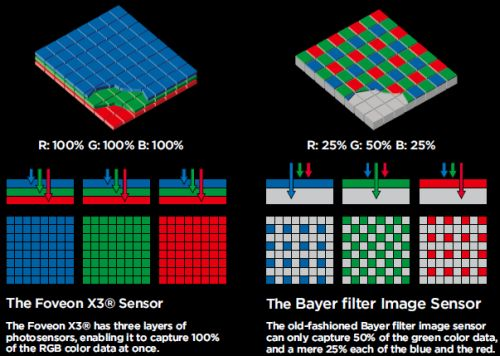
\includegraphics[scale=0.5]{images/L7_foveon_x3_Bayer.jpg}
\end{center}
\end{frame}
%---------------
\begin{frame}
\frametitle{Mono CCD}
\framesubtitle{Bayer pattern and Foveon X3}
\begin{columns}
\column{0.3\textwidth}
\begin{center}
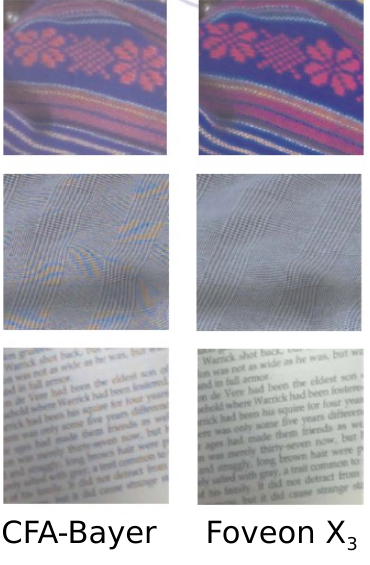
\includegraphics[scale=0.3]{images/L7_ex_FoevonBayer.png}
\end{center}
\column{0.7\textwidth}
\begin{center}
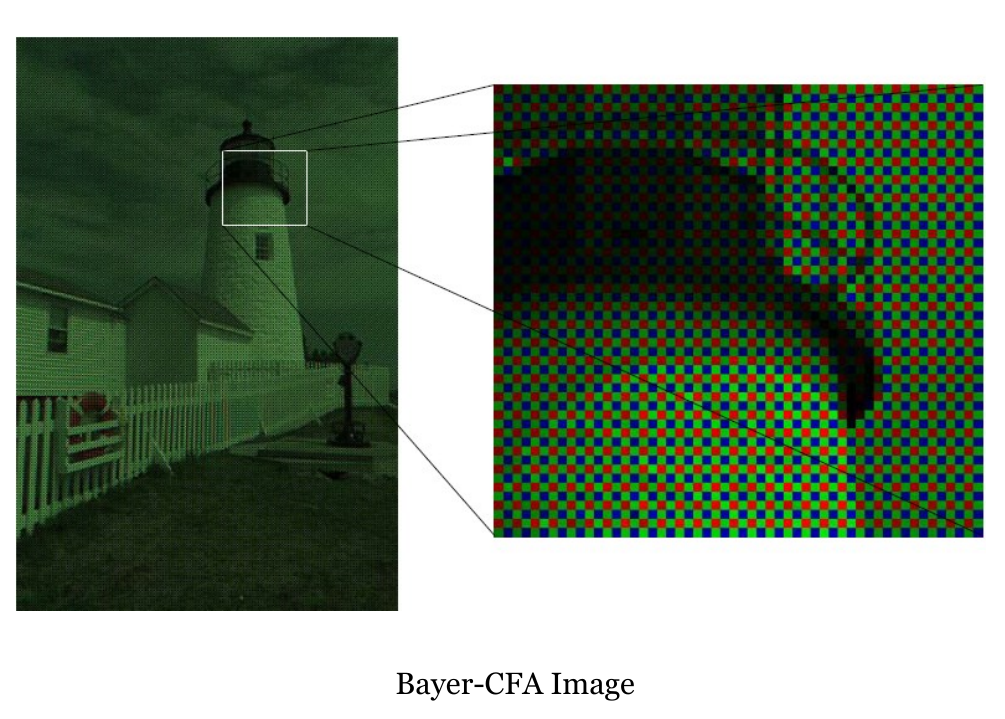
\includegraphics[scale=0.26]{images/L7_ex_BayerCFA}
\end{center}
\end{columns}
\end{frame}
%---------------
\section{Demosaicing}
\begin{frame}
\frametitle{Demosaicing}
\framesubtitle{Bayer Color filter Array (CFA) Image}
\scriptsize{ULR: Original, Red, BLR: Green and blue}
\begin{center}
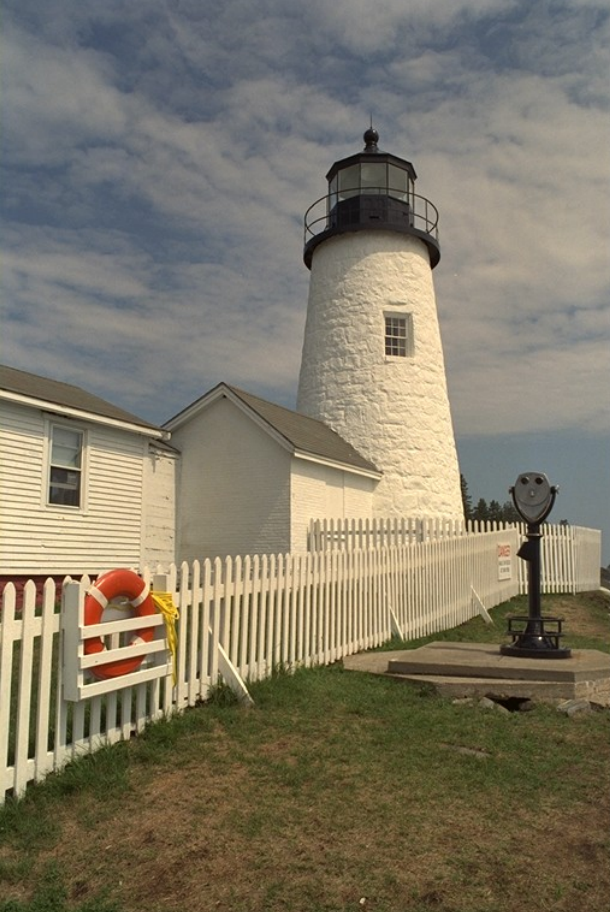
\includegraphics[width = 0.25\textwidth, height = 0.36\textheight]{images/L7_lighthouseOri.png}\
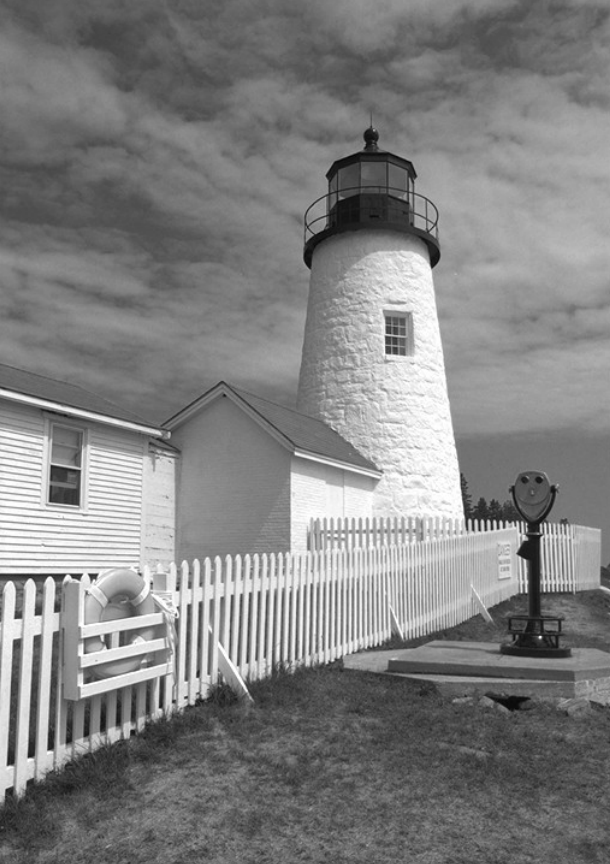
\includegraphics[width = 0.25\textwidth, height = 0.36\textheight]{images/L7_lighthouseRed.png}\\
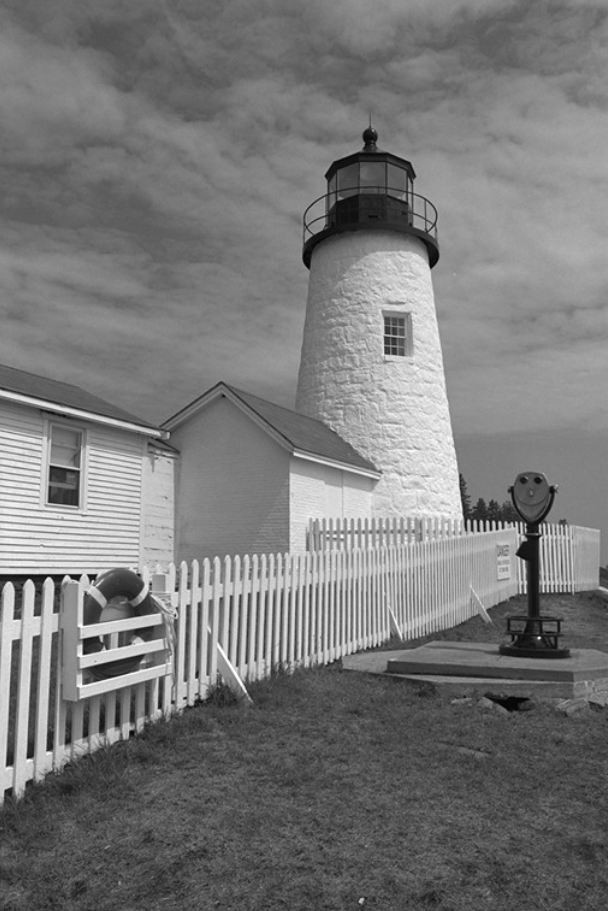
\includegraphics[width = 0.25\textwidth, height = 0.36\textheight]{images/L7_lighthouseGreen.png}\
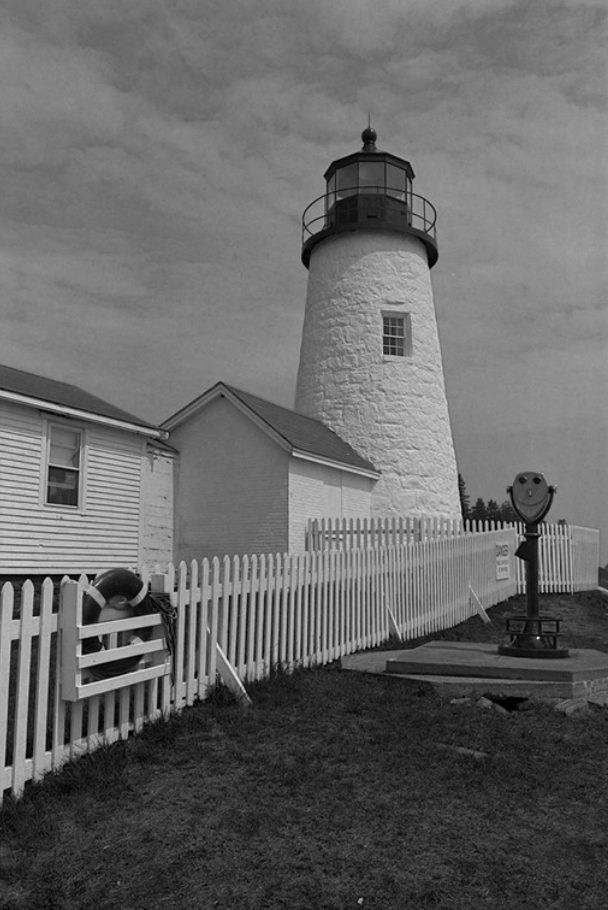
\includegraphics[width = 0.25\textwidth, height = 0.36\textheight]{images/L7_lighthouseBlue.png}
\end{center}
\end{frame}

%--------------
\begin{frame}
\frametitle{Demosaicing}
\framesubtitle{Bayer Color filter Array (CFA) Image}
\begin{center}
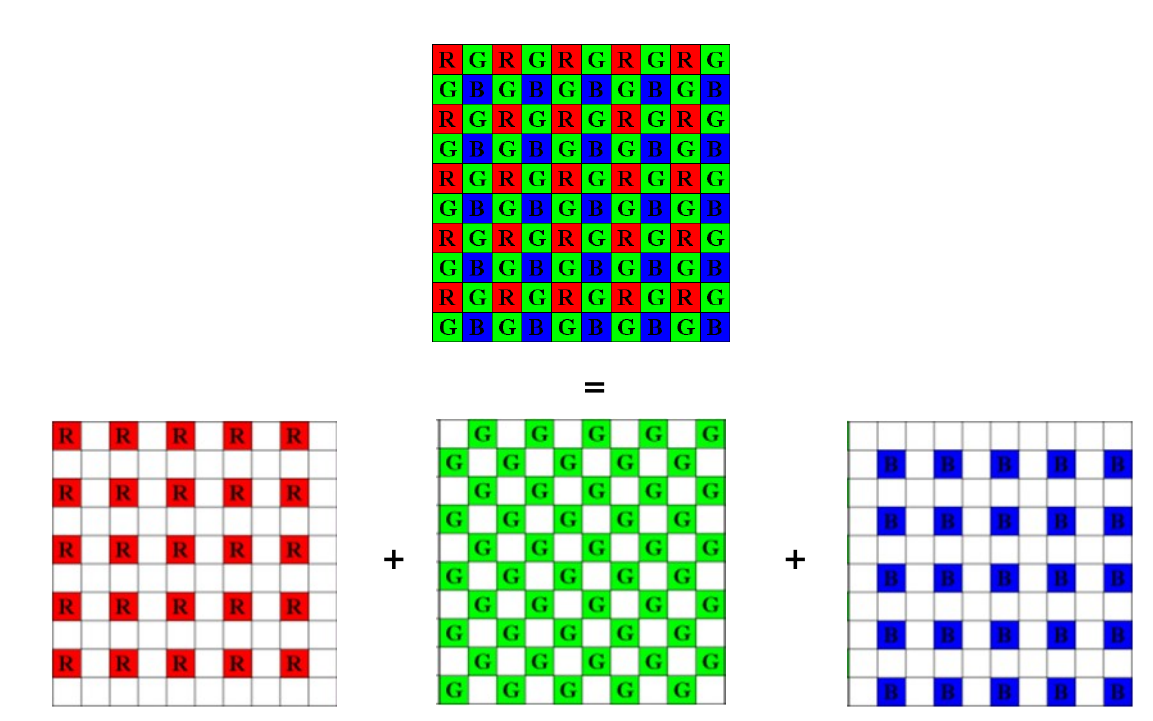
\includegraphics[scale=0.35]{images/L7_BayerSensor.png}
\end{center}
\end{frame}

\begin{frame}
\frametitle{Demosaicing}
\scriptsize{Original and Red}
\begin{center}
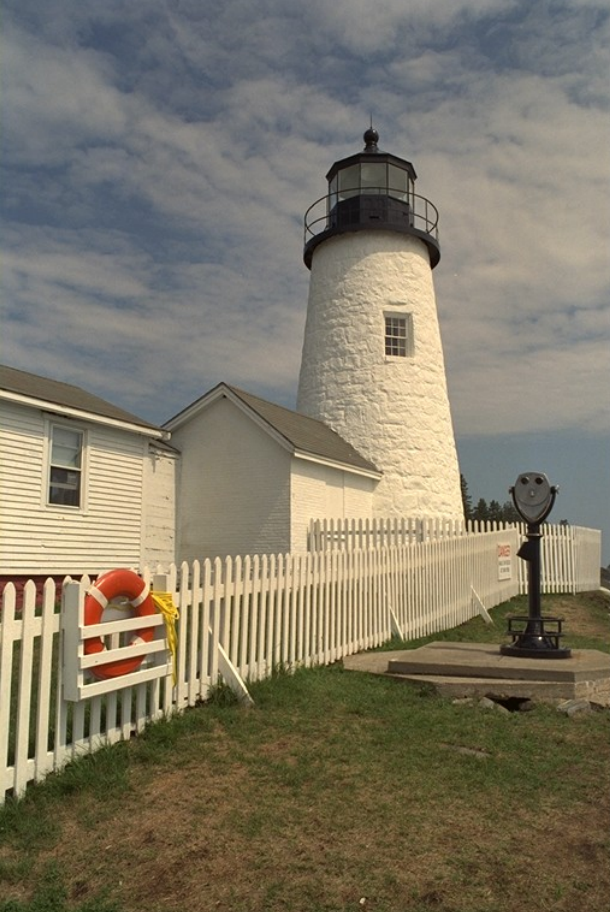
\includegraphics[width = 0.4\textwidth, height = 0.6\textheight]{images/L7_lighthouseOri.png}\
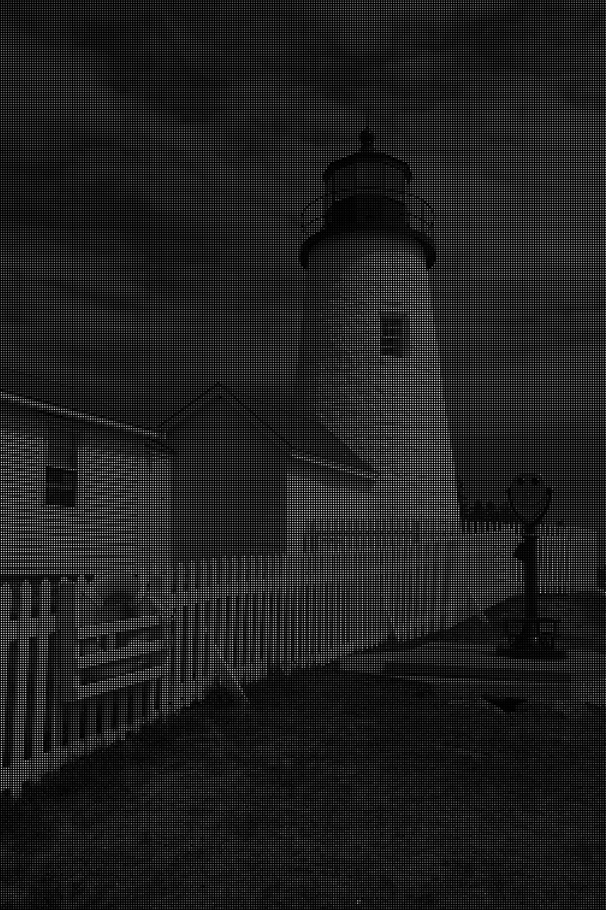
\includegraphics[width = 0.4\textwidth, height = 0.6\textheight]{images/L7_lighthouseRedSubSam.png}\
\end{center}
\end{frame}

\begin{frame}
\frametitle{Demosaicing}
\frametitle{Bayer Color filter Array (CFA) Image}
\scriptsize{Green and Blue}
\begin{center}
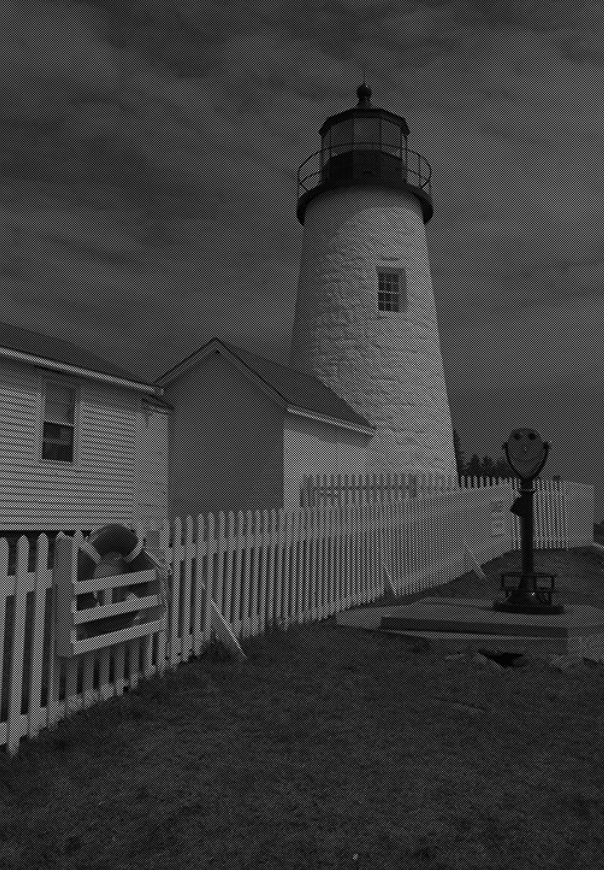
\includegraphics[width = 0.4\textwidth, height = 0.6\textheight]{images/L7_lighthouseGreenSubSam.png}\
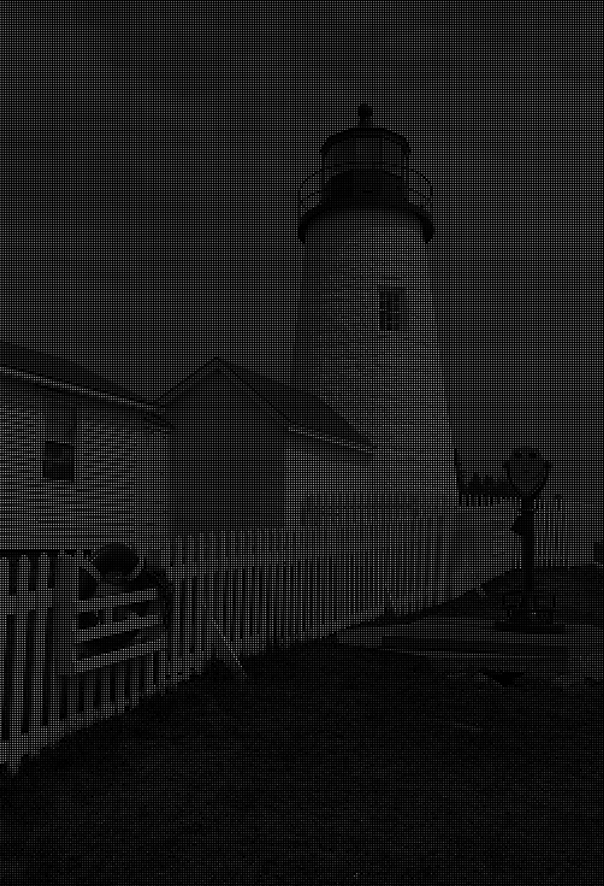
\includegraphics[width = 0.4\textwidth, height = 0.6\textheight]{images/L7_lighthouseBlueSubSam.png}
\end{center}
\end{frame}

\begin{frame}
\frametitle{Demosaicing}
\frametitle{Bayer Color filter Array (CFA) Image}
\scriptsize{Bayer CFA image}
\begin{center}
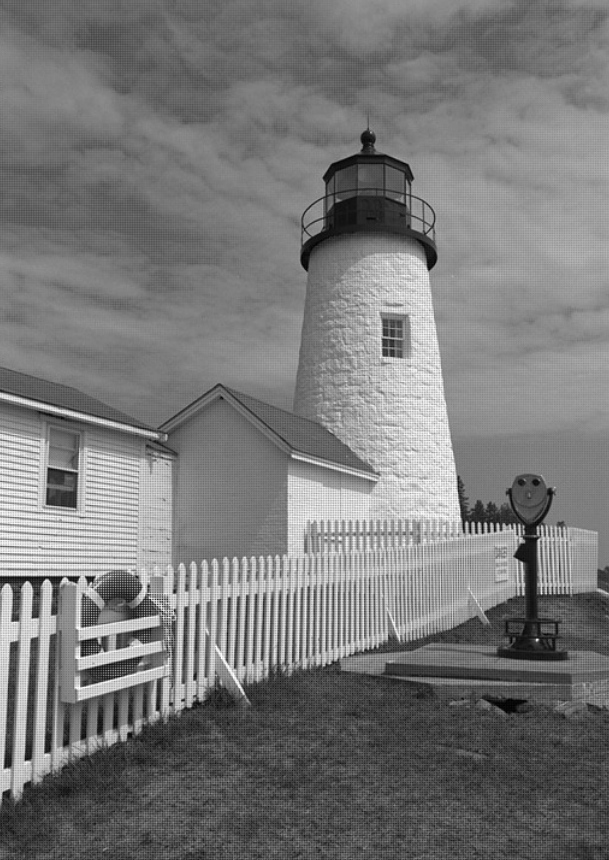
\includegraphics[width = 0.46\textwidth, height = 0.76\textheight]{images/L7_lighthouseBayerCFA.png}
\end{center}
\end{frame}

%---------------
\begin{frame}
\frametitle{Demosaicing}
\begin{block}{Techniques}
\begin{itemize}
\item Nearest neighbor replication 
\item Bilinear interpolation
\item Smooth Hue transition interpolation
\item Edge preserving interpolation
\item Pattern recognition interpolation
\end{itemize}
\end{block}
\end{frame}
%---------------
\begin{frame}
\frametitle{Demosaicing}
\framesubtitle{Nearest Neighbor Replication}
\begin{center}
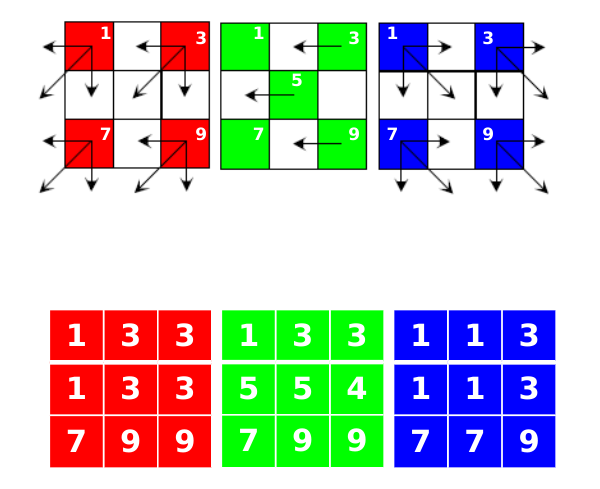
\includegraphics[scale=0.4]{images/L7_NN.png}
\end{center}
\end{frame}
\begin{frame}
\frametitle{Demosaicing}
\framesubtitle{Nearest Neighbor Replication}
\begin{block}{Result}
\begin{center}
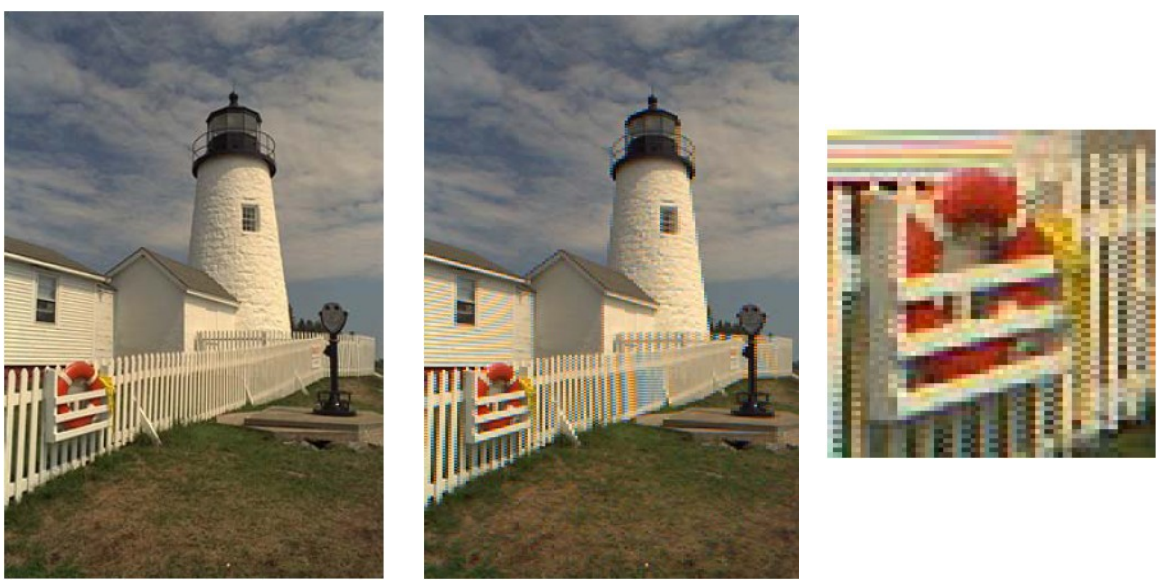
\includegraphics[scale=0.35]{images/L7_res_NN.png}
\end{center}
\end{block}
\end{frame}
%---------------
\begin{frame}
\frametitle{Demosaicing}
\framesubtitle{Bilinear Interpolation}
\begin{center}
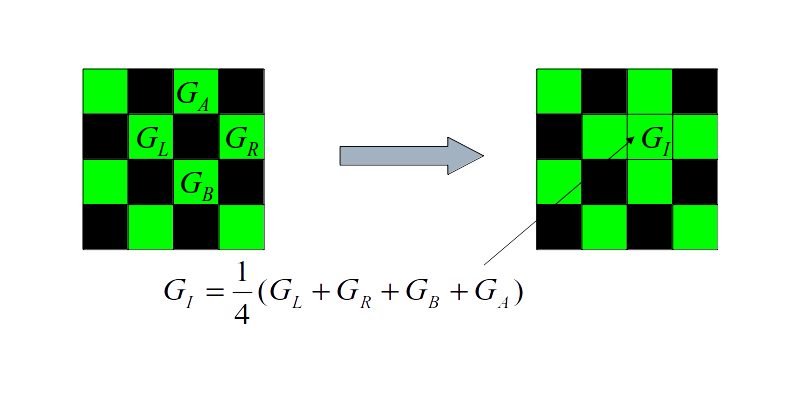
\includegraphics[scale=0.2]{images/L7_GreenBI2.png}\\
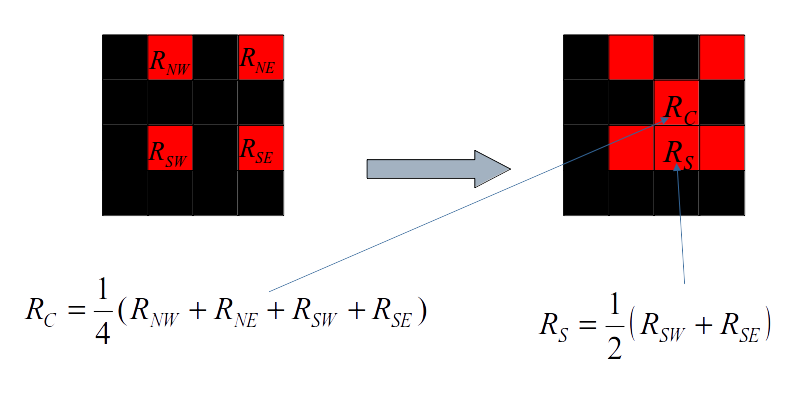
\includegraphics[scale=0.2]{images/L7_RedBI.png}
\end{center}
\end{frame}

\begin{frame}
\frametitle{Demosaicing}
\framesubtitle{Bilinear Interpolation}
\begin{block}{Result}
\begin{center}
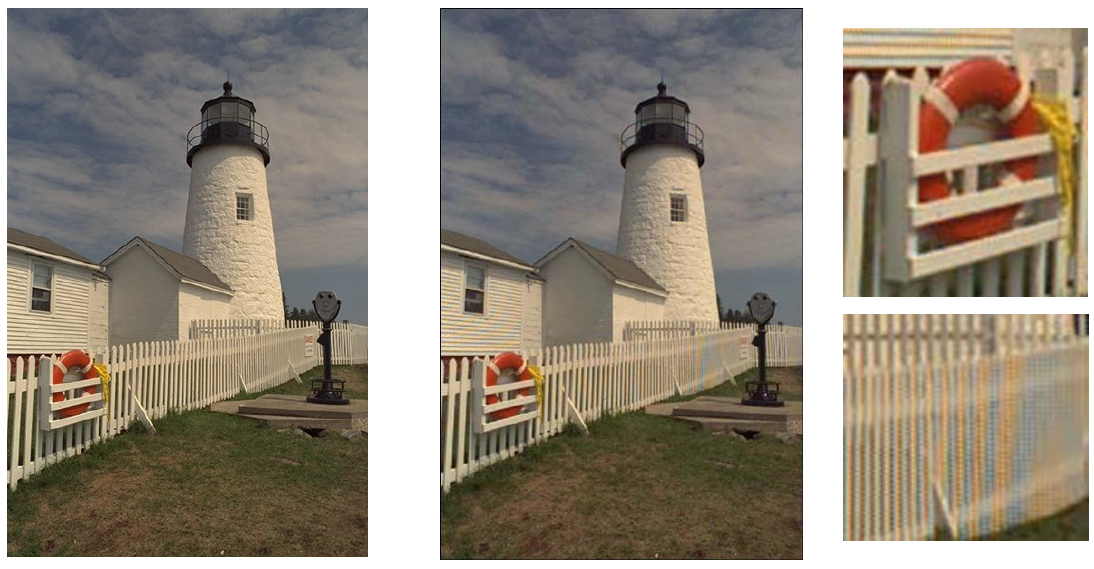
\includegraphics[scale=0.35]{images/L7_res_BI.png}
\end{center}
\end{block}
\end{frame}
%---------------
\begin{frame}
\frametitle{Demosaicing}
\framesubtitle{Smooth Hue Transition Interpolation}
\begin{itemize}
\item Impose smooth transition in hue from pixel to pixel $\rightarrow$ {\color{red}Red, hue values} = {\color{red}R}/{\color{green}G}, and 
{\color{blue}Blue, hue values} = {\color{blue}B}/{\color{green}G}
\item Interpolation of {\color{green} Green} pixels same as Bilinear interpolation 
\end{itemize}
\begin{center}
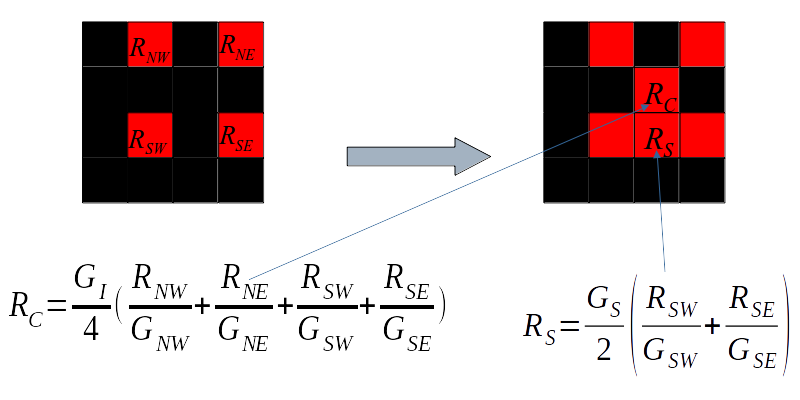
\includegraphics[scale=0.3]{images/L7_SmoothedCI.png}
\end{center}
\end{frame}

\begin{frame}
\frametitle{Demosaicing}
\framesubtitle{Smooth Hue Transition Interpolation}
\begin{block}{Result}
\begin{center}
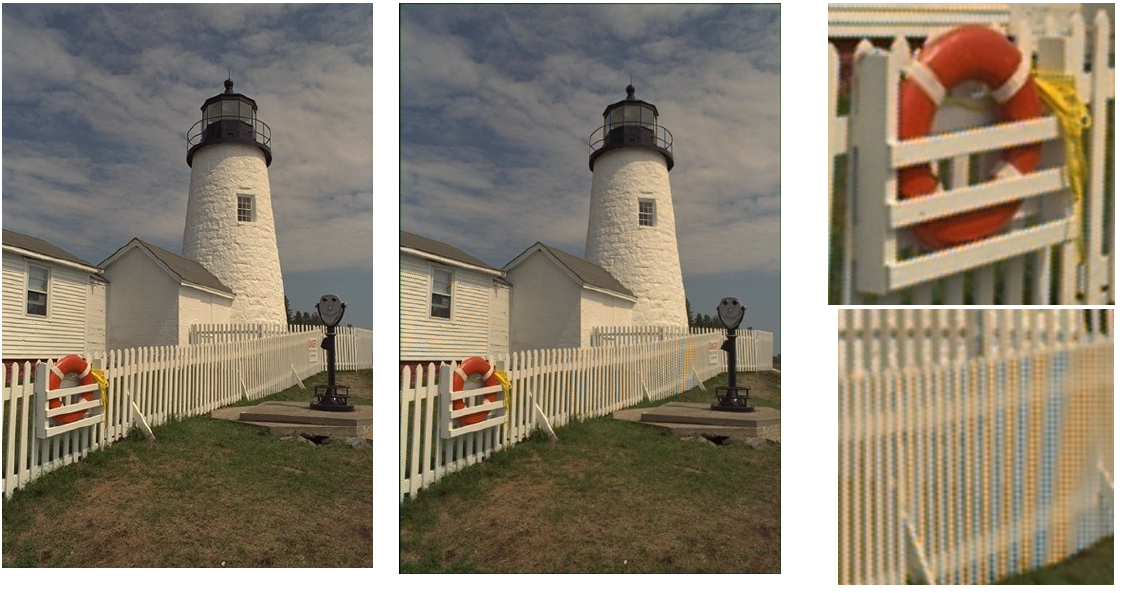
\includegraphics[scale=0.35]{images/L7_res_SHT.png}
\end{center}
\end{block}
\end{frame}
%---------------
\begin{frame}
\frametitle{Demosaicing}
\framesubtitle{Edge Preserving Interpolation}
\footnotesize{
\begin{itemize}
\item Interpolation of {\color{red} Red} / {\color{blue} Blue} pixels is the same as Smooth Hue Transition
\item Working with two gradient for the {\color{green} Green} pattern, one in horizontal direction and one in vertical direction
\item $ \Delta H = \vert G_{L} - G_{R}\vert $  and  $ \Delta V = \vert G_{A} - G_{B}  \vert $ 
\end{itemize}
}
\begin{columns}
\column{0.6\textwidth}
\footnotesize{
\begin{itemize}
\item[] If $\Delta H < \Delta V$ 
\scriptsize{
\begin{itemize}
	\item[] $G_{I} = (G_{L}+G_{R})/2$
\end{itemize}
}
\item[] Else if $\Delta H > \Delta V$ 
\scriptsize{
\begin{itemize}
	\item[] $G_{I} = (G_{A}+G_{B})/2$
\end{itemize}
}
\item[] Else
\scriptsize{
\begin{itemize}
	\item[] $G_{I} = (G_{L}+G_{R}+G_{A}+G_{B})/4$
\end{itemize}
}
\end{itemize}
}
\column{0.4\textwidth}
\centering{
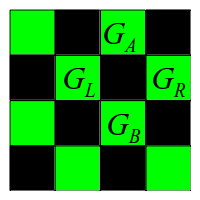
\includegraphics[scale=0.5]{images/L7_greenpixels.png}}
\end{columns}
\end{frame}

\begin{frame}
\frametitle{Demosaicing}
\framesubtitle{Edge Preserving Interpolation}
\begin{block}{Result}
\begin{center}
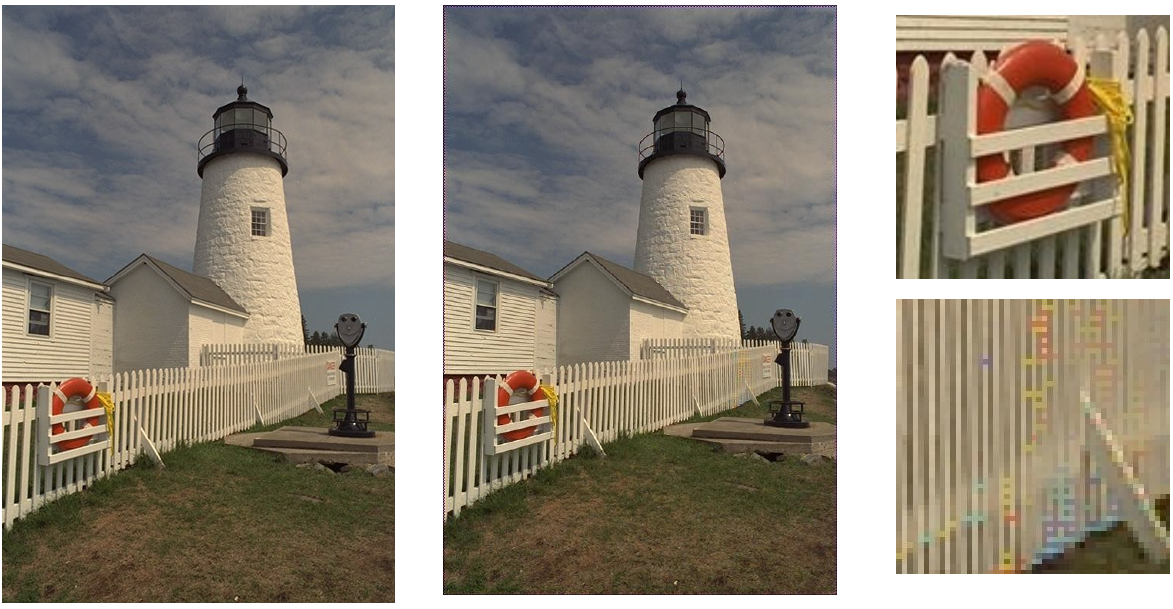
\includegraphics[scale=0.35]{images/L7_res_EPI.png}
\end{center}

\end{block}
\end{frame}

%----------------
\begin{frame}
\frametitle{Demosaicing}
\framesubtitle{Edge Preserving Interpolation \small{(larger neighborhood)}}
\footnotesize{
\begin{itemize}
\item Interpolation of {\color{red} Red} / {\color{blue} Blue} pixels is the same as Smooth Hue Transition
\item Horizontal gradient, $\Delta H = \vert G_{4} - G_{6}\vert + \vert R_{5} - R_{3} + R_{5} - R_{7} \vert $
\item Vertical gradient, $\Delta V = \vert G_{2} - G_{8}\vert + \vert R_{5} - R_{1} + R_{5} - R_{9} \vert $
\end{itemize}
}
\begin{columns}
\column{0.7\textwidth}
\footnotesize{
\begin{itemize}
\item[] If $\Delta H < \Delta V$ 
\scriptsize{
\begin{itemize}
	\item[] $G_{5} = (G_{4}+G_{6})/2 + (R_5-R_3+R_5-R_7)/4$
\end{itemize}
}
\item[] Else if $\Delta H > \Delta V$ 
\scriptsize{
\begin{itemize}
	\item[] $G_{5} =(G_{2}+G_{8})/2 + (R_{5}-R_{1}+R_{5}-R_{9})/4$
\end{itemize}
}
\item[] Else
\scriptsize{
\begin{itemize}
	\item[] $G_{I} = (G_{L}+G_{R}+G_{A}+G_{B})/4 + (R_{5}-R_{1}+R_{5}-R_{9}+R_{5}-R_{3}+R_{5}-R_{7})/8$
\end{itemize}
}
\end{itemize}
}
\column{0.3\textwidth}
\centering{
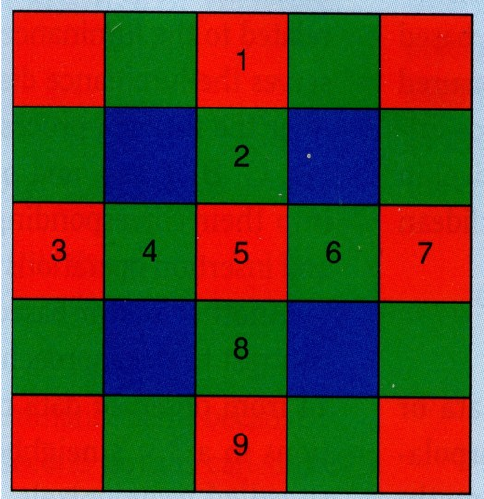
\includegraphics[scale=0.27]{images/L7_EPI_L.png}}
\end{columns}
\end{frame}

\begin{frame}
\frametitle{Demosaicing}
\framesubtitle{Edge Preserving Interpolation \small{(Larger neighborhood)}}
\begin{block}{Result}
\centering{
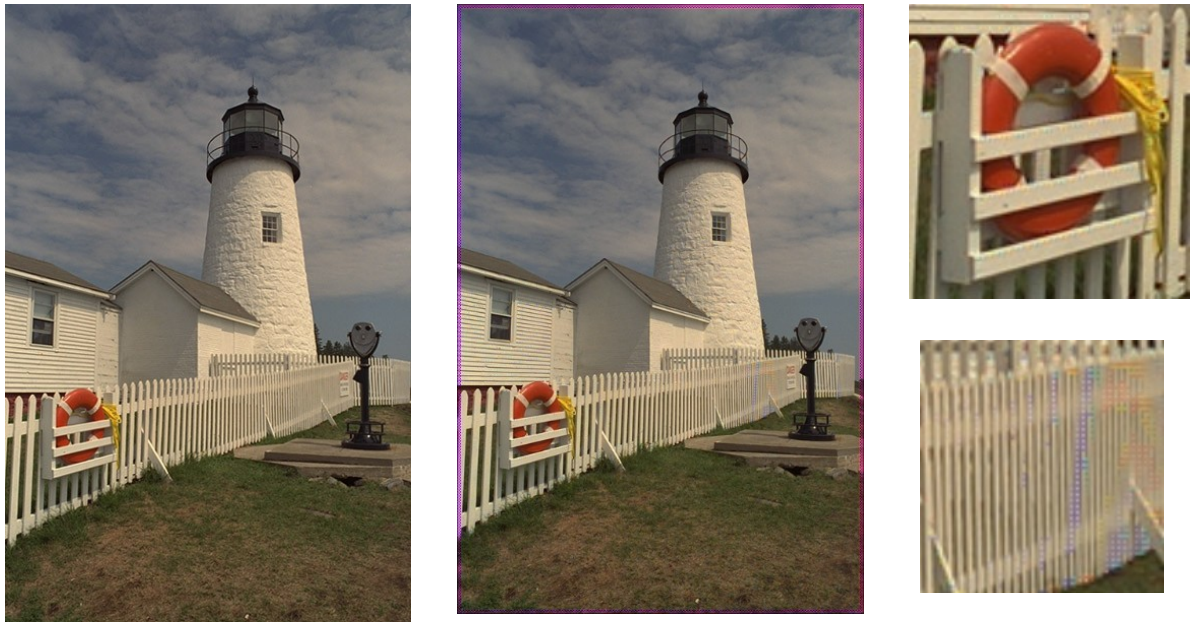
\includegraphics[scale=0.32]{images/L7_res_EPIL.png}}

\end{block}
\end{frame}
%------------
\begin{frame}
\frametitle{Demosaicing}
\framesubtitle{Pattern Recognition Interpolation}
\footnotesize{
\begin{itemize}
\item Interpolating the {\color{green}green} color plane considering three different edge type
\item Once the {\color{green}green} plane is interpolated, the {\color{red}red} and {\color{blue}blue} planes are interpolated using the Smooth Hue Transition
\item First: Classifying the four neighborhood and low $L$ or high $H$ in comparison to their average
\item Edge: if three neighbor pixel share the same classification (Low and High edge, respectively)\\
\end{itemize}
}
\begin{center}
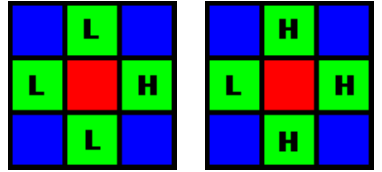
\includegraphics[scale=0.33]{images/L7_PRI_Edge.png}
\end{center}
\end{frame}
%-------------
\begin{frame}
\frametitle{Demosaicing}
\framesubtitle{Edge Preserving Interpolation \small{(Larger neighborhood)}}

\footnotesize{
\begin{itemize}
\item Corner: if two adjacent neighbor pixels have the same classification
\end{itemize}
}
\begin{center}
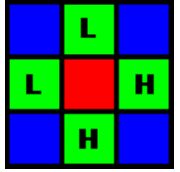
\includegraphics[scale=0.33]{images/L7_PRI_Corner.png}
\end{center}

\footnotesize{
\begin{itemize}
\item Stripe: if two opposite pixels have the same classification 
\end{itemize}
}
\begin{center}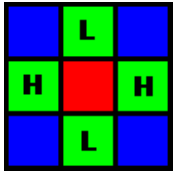
\includegraphics[scale=0.33]{images/L7_PRI_Stripe.png}\end{center}
\end{frame}
%-----------
\begin{frame}
\frametitle{Demosaicing}
\framesubtitle{Edge Preserving Interpolation \small{(Larger neighborhood)}}
\begin{itemize}
\item Edge pixel:
\begin{itemize}
\item $G_{I} = $ median$\{$ $G_{R},G_{L},G_{A},G_{B}$ $\}$
\item If we sort the neighbors $\{$ $G_{R},G_{L},G_{A},G_{B}$ $\}$ as $A>B>C>D$
\item $G_{I} = (B+C)/2$
\end{itemize}
\item Clip function for calculating the corner and stripe values
\item[]
\[
clip^{B}_{C}(x)=
\begin{cases}
B & x > B\\
x & C \leq x \leq B\\
C & x < C
\end{cases}
\]
\end{itemize}
\end{frame}

\begin{frame}
\frametitle{Demosaicing}
\framesubtitle{Edge Preserving Interpolation \small{(Larger neighborhood)}}
\begin{itemize}
\item Corner and Stripe pixel:
\begin{itemize}
\item $G_{I} = clip^{B}_{C}(2M -S)$
\item $M$ median of $H$ and $L$ pixels 
\item $S$ average of $X$ pixels in the neighborhood
\end{itemize}
\item[]
\centering{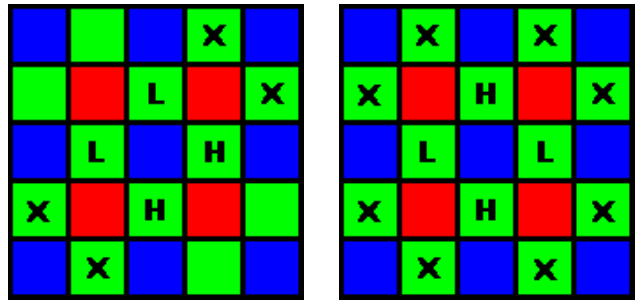
\includegraphics[scale=0.3]{images/L7_CornerStripe.png}}
\end{itemize}
\end{frame}

\begin{frame}
\frametitle{Demosaicing}
\framesubtitle{Edge Preserving Interpolation \small{(Larger neighborhood)}}
\begin{block}{Result}
\begin{center}
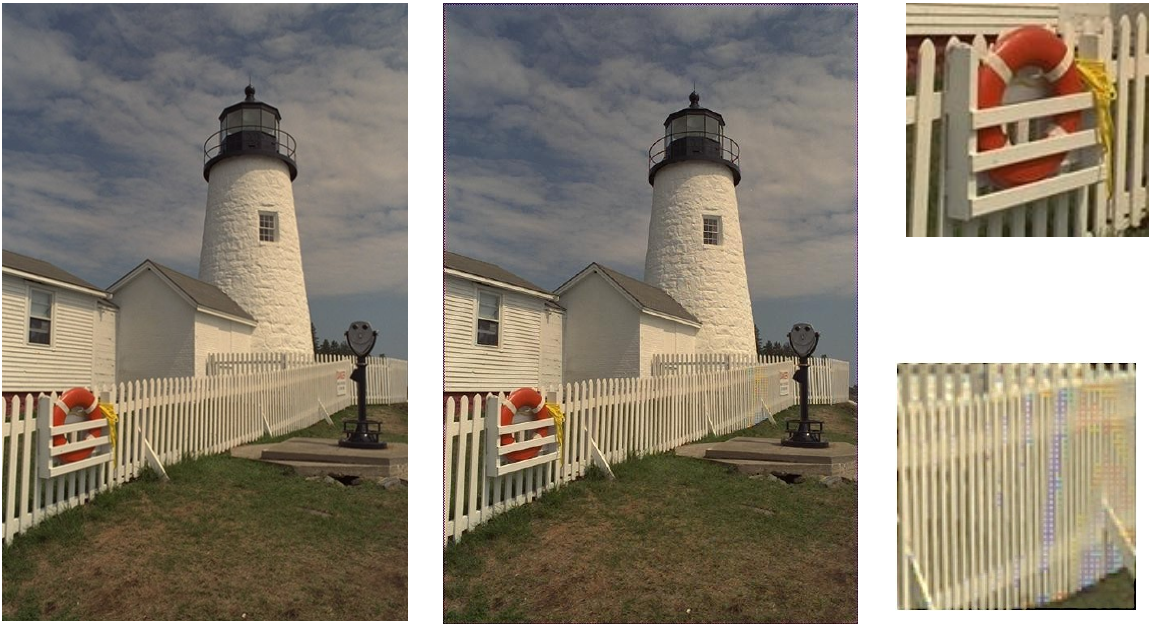
\includegraphics[scale=0.33]{images/L7_res_PRI.png}
\end{center}

\end{block}
\end{frame}
%-----------
%%% It need more reading and work, ----> This weekend 
%\section{Color Constancy}
%\begin{frame}
%\frametitle{Color Constancy}
%\begin{itemize}
%\item Human vision systems perceives stable light even with different ambient illumination
%\item {\color{blue} Of course Not the case of the cameras !!}
%\item From left to right: Canon S400, HP850, Nikon D1, and cellphone Nokia 6820 integrated camera 
%\end{itemize}
%\begin{center}
%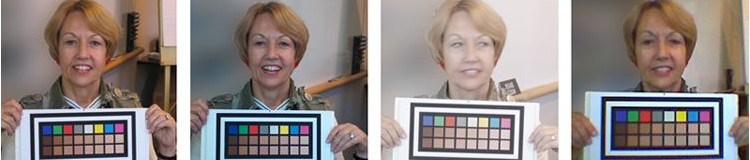
\includegraphics[width = 1.0\textwidth]{images/L7_DiffCamera2.jpg}
%\end{center}
%\end{frame}
%
%\begin{frame}
%\frametitle{Color Constancy}
%\begin{itemize}
%\item From left to right, scenes under illuminations: fluorescent daylight D65, incandescent A, and two fluorescent illumiants TL83 and TL84.\end{itemize}
%\begin{center}
%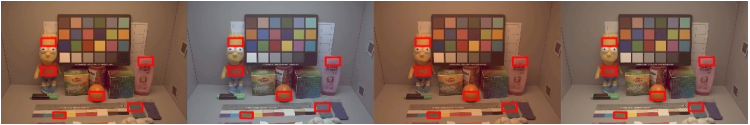
\includegraphics[width = 1.0\textwidth, height = 0.3\textheight]{images/L7_DiffLight2.png}
%\end{center}
%\end{frame}
%
%\begin{frame}
%\frametitle{Color Constancy}
%
%\end{frame}

\end{document}

%\begin{itemize}
%\item Also use neighborhood but do not use coefficients 
%\begin{itemize}
%\item median filter for noise reduction
%\end{itemize} 
%\end{itemize}
